\documentclass[10pt, a4paper]{article}

\usepackage[twocolumn,textwidth=16cm,columnsep=1cm]{geometry}
\usepackage[utf8]{inputenc}
\usepackage[english]{babel}
\usepackage{graphicx}
\usepackage{biblatex}
\usepackage{hyperref}
\usepackage[acronym]{glossaries}
\usepackage{titling}
\usepackage{minted}
\usepackage{markdown}
\usepackage{csquotes}
\usepackage{todonotes}
\usepackage{verbatim}

\addbibresource{references.bib}

\title{Thickshake: Towards A Smarter Library Catalogue}
\author{Mark Shelton}
\date{\today}

\newacronym{slwa}{SLWA}{State Library of Western Australia}
\newacronym{rdbms}{RDBMS}{Relational Database Management System}
\newacronym{orm}{ORM}{Object Relational Mapper}

\frenchspacing
\righthyphenmin2
\sloppy

\begin{document}

\begin{titlepage}
  \centering
  
\includegraphics[width=0.5\textwidth]{figures/pawsey}\par\vspace{1cm}
  {\scshape\LARGE Pawsey Supercomputing Centre \par}\vspace{0.5cm}
  {\scshape\Large Summer Internship Program (2017-18) \par}\vspace{2cm}
  {\LARGE\bfseries\thetitle\par}\vspace{2cm}
  {\Large\theauthor\par}\vfill
  {\large\em Supervised by\par}\vspace{0.5cm}
  Joshua Hollick, Curtin HIVE\par
  Dr.~Andrew Woods, Curtin HIVE\par
  Debra Jones, State Library of Western Australia\vfill
  {\large\thedate\par}
\end{titlepage}

\begin{abstract}
Modern computing technology allows for new insight into large photographic archives. We have developed Thickshake, a software package that can automatically generate and augment metadata for photographic archive items. Thickshake provides  four contributions: 1. A flexible interface to MARC-based library catalogues, 2. A metadata parsing framework (e.g. geolocation, date extraction), 3. An image processing framework (e.g. face detection, text extraction), and 4. A machine learning framework (e.g. subject recognition, landmark recognition). The system was developed and tested with a set of 10,106 images provided by the State Library of Western Australia and processed at the Pawsey Supercomputing Centre. Source code available here: \url{github.com/markshelton/thickshake}.
\end{abstract}

\section{Introduction}
\label{section:introduction}

The \Gls{slwa} is home to an archival image database consisting of approximately 700,000 pictures of Perth and the greater Western Australia region. These images are grouped as database entries for each set donated to the \Gls{slwa}, along with metadata pertaining to information such as the photographer, subject, location, and description. This metadata is manually produced by historians, volunteers, and photographers. This task is expensive and time-consuming for libraries, and does not necessarily provide the level of detail desired by end-users. Accessing databases like the \Gls{slwa} image archives via metadata text search has been described as failing to meet the scale and richness of the digital collection \cite{whitelaw2015}. Recent advances in technology have opened the possibility of automating archival image description, with potential benefits to efficiency and quality. We have developed Thickshake, a software system that generates and augments library catalogue metadata (\ref{figure:architecture}). Thickshake has four primary functions: a library interface (Section \ref{section:library_interface}), metadata parsing framework (Section \ref{section:metadata_parsing}), image processing framework (Section \ref{section:image_processing}), and machine learning framework (Section \ref{section:machine_learning}). 

\begin{figure}[ht]
  \centering
  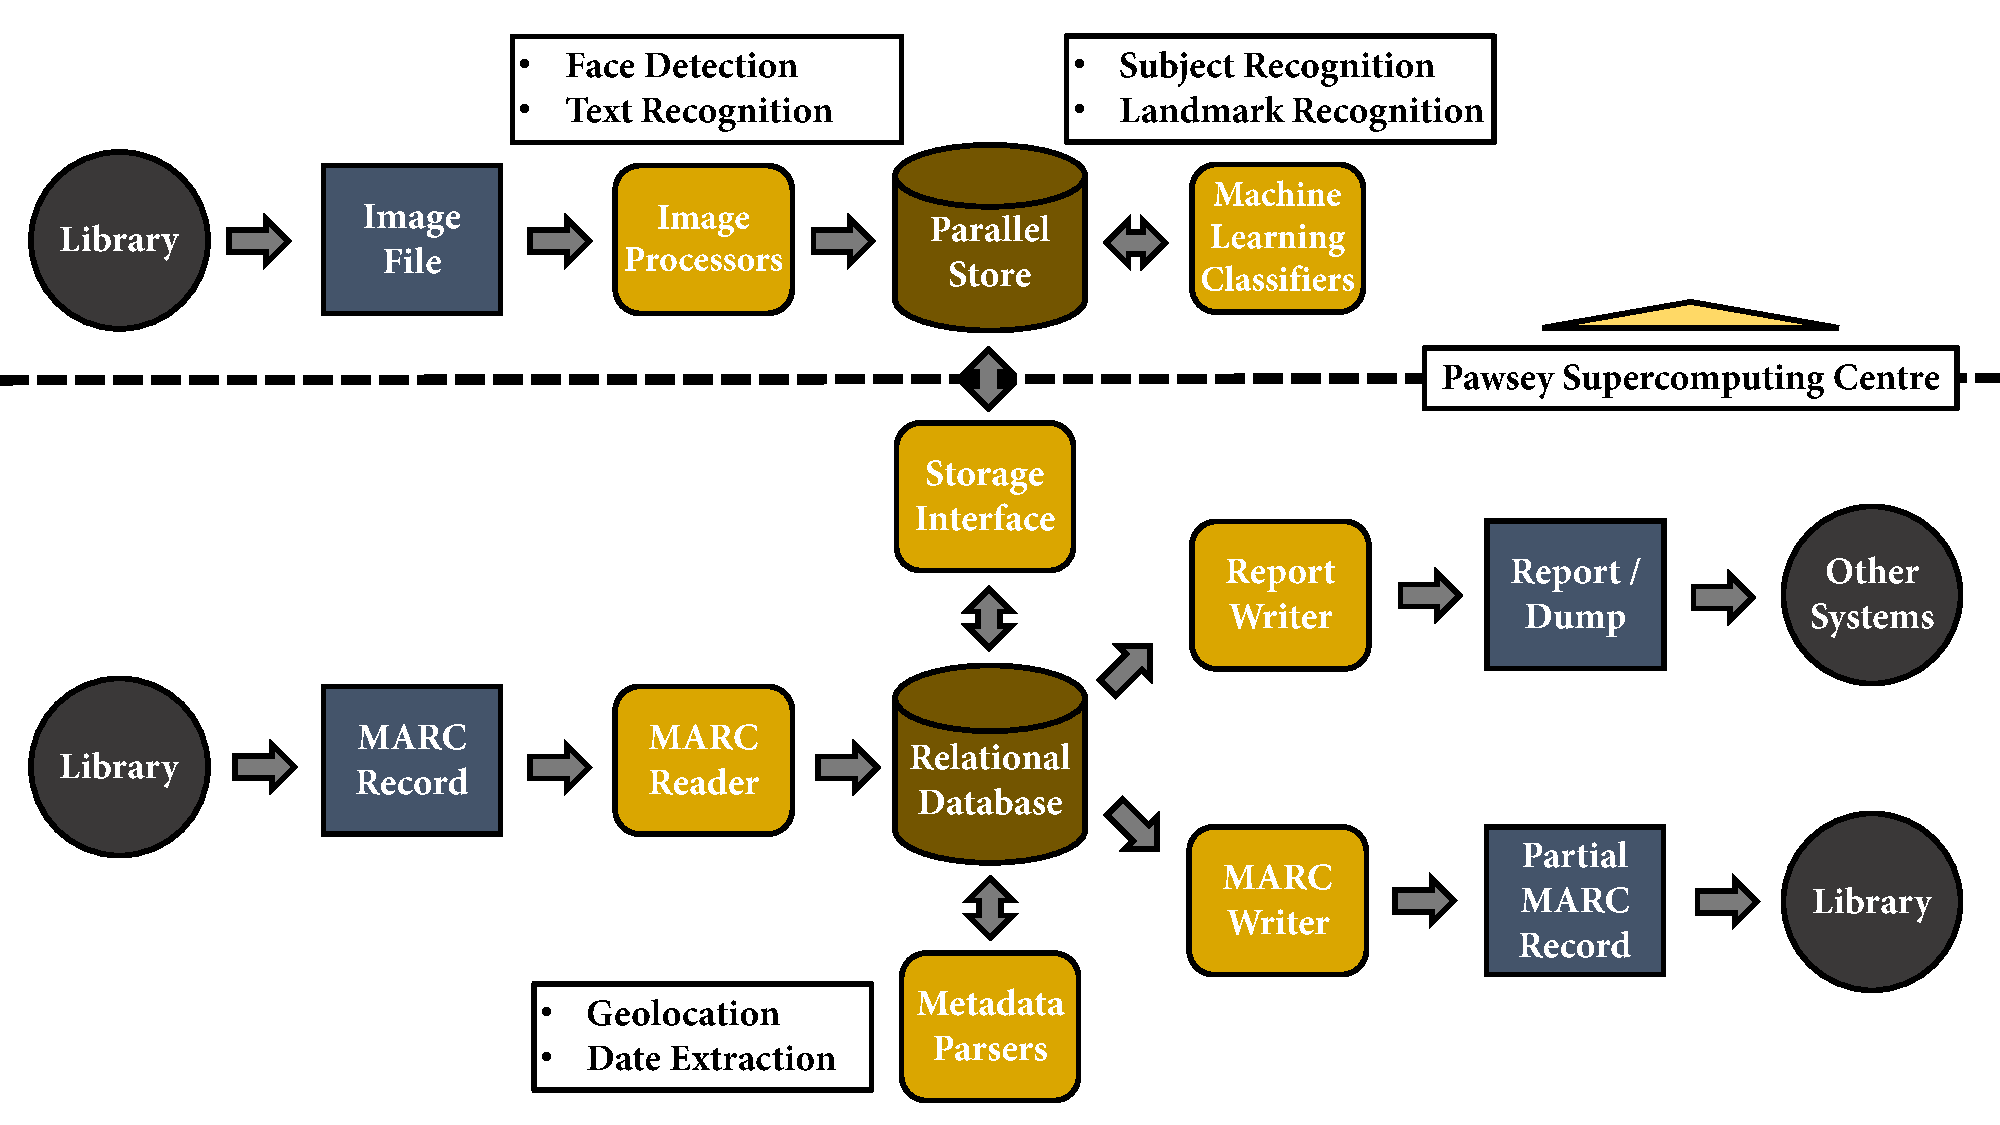
\includegraphics[width=\columnwidth]{figures/architecture}
  \caption{Thickshake system architecture.}
  \label{figure:architecture}
\end{figure}

\section{Library Interface}
\label{section:library_interface}

%\subsection{Introduction}
\label{subsection:library_interface:introduction}
MARC is the established international digital format for library materials. MARC records contain items' titles, subjects, topics, and other cataloguing details. However, MARC is complex and difficult to use. With an increasing quantity of resources to describe and catalogue, working with MARC records one-by-one is challenging. Cataloguers who work with MARC records in traditional library settings are now finding that they may need a new approach, one that combines traditional cataloguing and programming, in order to efficiently manage their work-flows. To address this shortcoming, we developed a system that maps MARC records onto a relational database, to facilitate easier querying, editing and reporting.

\subsection{MARC Importer}
\label{subsection:library_interface:marc_importer}
We leveraged Pymarc \cite{pymarc} to read and convert MARC files (JSON, XML, MARC21) into Python objects. Thickshake reads in a user-defined file that maps MARC codes to the tables and columns of a relational database (see Appendix \ref{appendix:marc_input_map}). The parser works through the mapping file recursively and tracks and creates relationships between tables in the database. This parser is generalisable to almost any mapping configuration and database schema, including cyclical relationships and table aliases. It takes approximately 11 minutes for the importer to load our test dataset (3,048 records; 10,106 images) into the database.

\subsection{Relational Database}
\label{subsection:library_interface:relational_database}
Thickshake connects to a relational database using the SQLAlchemy \Gls{orm}, which provides an abstracted high-level database execution wrapper. SQLAlchemy \Gls{orm} is compatible with a variety of \Gls{rdbms}, which can be swapped out depending on the application. For developing Thickshake we used PostgreSQL, which is free, open-source and implements most of the SQL standard. We used Docker (a lightweight virtualization tool) to containerize Thickshake. Docker creates a private virtual network that contains one Docker container hosting the application, and another Docker container hosting the PostgreSQL server (see Appendix \ref{appendix:docker_automated_build}). The database schema can be found in Appendix \ref{appendix:database_schema}. The base schema (inherited by the other tables) has a number of custom mixins: auto-generated table IDs, created\_at and modified\_at timestamps, and a permissive constructor. We also included dynamic fields that (on update) count the number of relationships between tables.

\subsection{MARC Exporter}
\label{subsection:library_interface:marc_exporter}
Thickshake can also create partial MARC records that can be loaded back into the library catalogue. Similar to the MARC import process, Thickshake reads in a user-defined file that maps the relational database to MARC codes (see Appendix \ref{appendix:marc_output_map}). As Thickshake's MARC import process does not guarantee the preservation of all the information stored in MARC (this is dependent on the mapping file), we cannot export a full replica of the original MARC file. However, we can export a partial record with the augmented / desired fields along with identifying record and image labels. The \Gls{slwa} systems can import and merge these partial records into the existing catalogue. This functionality is planned but incomplete.

\subsection{Report Exporter}
\label{subsection:library_interface:report_exporter}
Thickshake can also produce reports in formats (e.g. CSV, JSON, HDF5) for use in other systems. As Thickshake is backed onto a \Gls{rdbms}, most standard SQL queries can be executed directly against the database, called by other functions or executed through the command-line interface. For example, this functionality is leveraged by the OldPerth project (also developed by our research group, not yet published), a historical photo geolocation website derived from OldNYC \cite{oldnyc}. OldPerth's workflow involves loading the \Gls{slwa} catalogue into Thickshake, running the geolocation metadata parser (see Section \ref{subsection:metadata_parsing:geolocation}), and then exporting the records into a CSV file. Large flat-file dumps can also be generated by performing left outer joins across the tables in the database, for use in machine learning.

\section{Metadata Parsing}
\label{section:metadata_parsing}

%\subsection{Introduction}
\label{subsection:metadata_parsing:introduction}
MARC fields were originally designed to be machine-readable but they are relatively unstructured by modern computing standards. For example, a MARC record's image note field (856z) usually contains an image's identifier code, title, location, and date - all in one text string. We have developed a metadata parsing framework to extract useful, structured information from semi-structured MARC fields and load the new data back into the database. We have developed parsers to perform geolocation, date extraction, and image dimension extraction.

\subsection{Framework}
\label{subsection:metadata_parsing:framework}
The metadata parsing framework we developed wraps around parsing functions to apply them to Thickshake's relational database. As arguments, the wrapper takes the parsing function, the table and columns of the input data, the intended output table, and an output map (that maps the intermediate dictionary to output table columns). Custom parsing functions simply require a signature that takes a list of values or a single value and returns a dictionary. The metadata parser operates on one record at a time, saving each record to the database as it is processed.

\subsection{Geolocation}
\label{subsection:metadata_parsing:geolocation}
The physical location of an image is useful for clustering, searching and visually representing historical archives. However, GPS coordinates are rarely stored in the \Gls{slwa} catalogue. We built a geolocation parser that parses a structured location from an image's note field (856z) and uses a geocoding service to convert that structured location into a qualified address and GPS coordinates. The image note field is usually of the structure: "identifier: title, location, date". The ideal location string is of the structure "street\_number street\_name street\_type, suburb\_name" but often deviates from this structure. We use regex pattern matching to loosely match these components and created a structured dictionary of location terms. We then use the Mappify.io API to geocode these structured locations into the closest qualified addresses, which also include GPS coordinates \cite{mappify}. We tested this system on 1,293 images sampled from our test set (we took a sample because Mappify.io has a daily rate-limit of 2,500 queries per day). Of the 1,293 images we attempted to parse, 260 (20\%) could be geocoded successfully (i.e. given GPS coordinates), and another 273 (21\%) could not be geocoded but could be parsed (i.e. given a structured address). The remaining 760 images (59\%) either did not contain location text in their image note or had complicated image note text that could not be parsed. We used this system in our OldPerth project to place \Gls{slwa} photos on an interactive map (see Figure~\ref{figure:oldperth}).

\begin{figure}[ht]
  \centering
  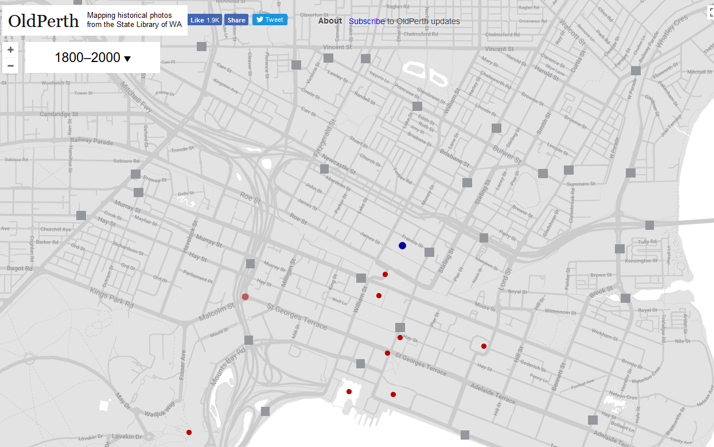
\includegraphics[width=\columnwidth]{figures/oldperth.png}
  \caption{Screenshot of OldPerth prototype. Red and blue dots represent geo-located photographs.}
  \label{figure:oldperth}
\end{figure}

\subsection{Date Extraction}
\label{subsection:metadata_parsing:date_extraction}
Dates are useful for tying images and their subjects together (e.g. in subject recognition, image clustering), but only if they are stored in a consistent and comparable format. We built a parser to handle extracting dates from different text fields in MARC records. The primary date parser returns a list of all dates found in a list of given strings. We transform the result of this primary parser to achieve different results, for example, we use it to extract a single date from an image's note field (856z) and we also use it to split a subject's date range field (100d) into separate start and end dates. The parser extracts potential dates from text using a combination of regex pattern matching and an external library, Datefinder \cite{datefinder}. The parser handles partial dates by filling in the unknown components with default values. Of the 10,106 images in our test dataset, we were able to extract date values from the image notes of 9,155 (91\%), and of these 5,770 (63\%) had all three day, month and year values (i.e. no default values were used). Parsing our test dataset to extract dates from image notes took approximately 5 minutes.

\subsection{Image Dimensions}
\label{subsection:metadata_parsing:image_dimensions}
Finally, we built a parser to extract image dimensions from image URL fields (856u). This parser is used in our OldPerth mapping project and could be potentially used in other visualisation exercises. Downloading the entire image and then checking the dimensions wastes time, bandwidth, and memory. Instead, our image dimension parser loads just enough of the image to be able to determine the dimensions. We use the Requests HTTP library to open a binary stream of the image \cite{requests}. We iterate over the binary stream loading it in chunks which we attempt to parse using the Pillow image manipulation library \cite{pillow}. As soon as enough of the image is parsed to allow the dimensions to be determined (normally this metadata is stored at the beginning of the stream) the stream terminates.

\section{Image Processing}
\label{section:image_processing}

%\subsection{Introduction}
\label{subsection:image_processing:introduction}
While the metadata parsers described in the previous section are able to augment existing metadata, image processing can reduce the need for manual description altogether. Images are a rich source of metadata, but processing them is computationally intensive. We have developed an image processing framework that is designed for a distributed, high-performance computing environment, specifically, Pawsey Supercomputing Centre’s Athena GPU cluster. Image processing results are stored in a parallel-access HDF5 store which our system syncs with the main relational database (see Section \ref{subsection:machine_learning:parallel_datastore}). We have developed two image processing functions that work within this framework: face detection and text recognition.

\subsection{Face Detection}
\label{subsection:image_processing:face_detection}
When researchers use the \Gls{slwa} catalogue (or similar photo collections), a common goal is to identify and track people of interest. Pre-empting this aim, library staff attempt to identify the subjects of the photos when they initially enter them into the catalogue (often referring to other historical records). However, this task is challenging and time-consuming. We developed an image processing function that automatically detects faces in photos. In a later section, we discuss how this could be used as part of automated subject recognition (see Section \ref{subsection:machine_learning:subject_recognition}).

The face detection function leverages two external libraries: Dlib \cite{dlib} and OpenCV \cite{opencv}. First, we load and pre-process each image using OpenCV's Contrast Limited Adaptive Histogram Equalization (CLAHE) function on each channel of the image to enhance the local contrast across the image \cite{opencv_clahe}. Second, we use Dlib's face detector function, which is made using Histogram of Oriented Gradients (HOG) combined with a linear classifier, an image pyramid, and a sliding window detection scheme \cite{dlib_face}. The output of this function is a list of bounding box coordinates for each face detected.

\begin{figure}[ht]
  \centering
  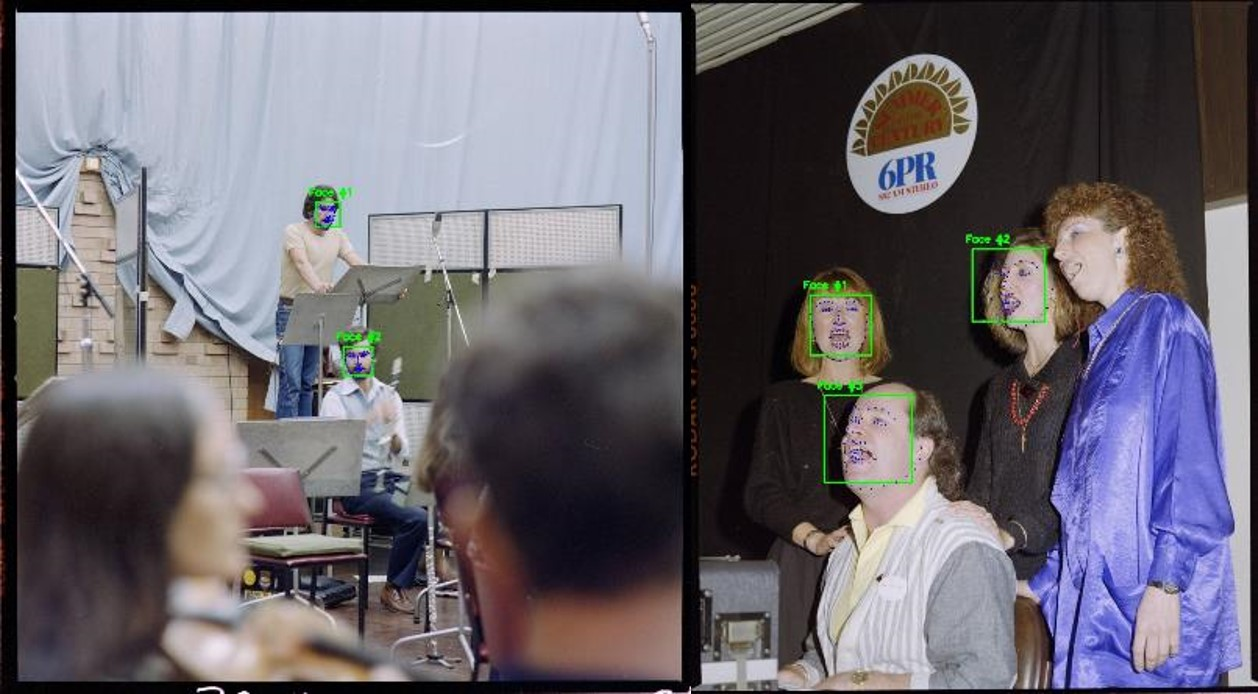
\includegraphics[width=\columnwidth]{figures/face_detection.jpg}
  \caption{Two photographs processed with Thickshake's face detection algorithm. Green boxes are the bounding boxes of each detected face. Blue dots are the detected facial landmarks.}
  \label{figure:face_detection:images}
\end{figure}

\subsection{Text Recognition}
\label{subsection:image_processing:text_recognition}
Embedded text can provide useful information about the context or content of an image. Text may be present in the original photo itself (e.g. a building sign) or placed on the physical medium (e.g. written notes). We developed a text recognition function to detect this embedded text, built on OpenCV's character recognition tools and Google's Tesseract library. While Tesseract is an excellent text recognition tool, it was primarily designed to read printed text from scanned documents (e.g. a book) \cite{tesseract}. In our test set, few of these images exist. To adapt Tesseract to extract handwritten text or text embedded in scenery, we developed a multi-stage pre-processing system. First, we use OpenCV's scene text detection (based on Class-specific Extremal Regions) to detect all regions that may contain text \cite{opencv_text}. Second, we apply a pre-processing optimisation system to each region using Hyperopt. Hyperopt is a Python library for serial and parallel optimization over awkward search spaces, which may include real-valued, discrete, and conditional dimensions \cite{hyperopt}. The pre-processing involves adding bleed to the detected region and then applying a binary thresholder. Hyperopt alters both the quantity of bleed and the binary threshold, to optimise for a result that has the highest amount of valid words (as a percentage) in the detected string.

\begin{figure}[ht]
  \centering
  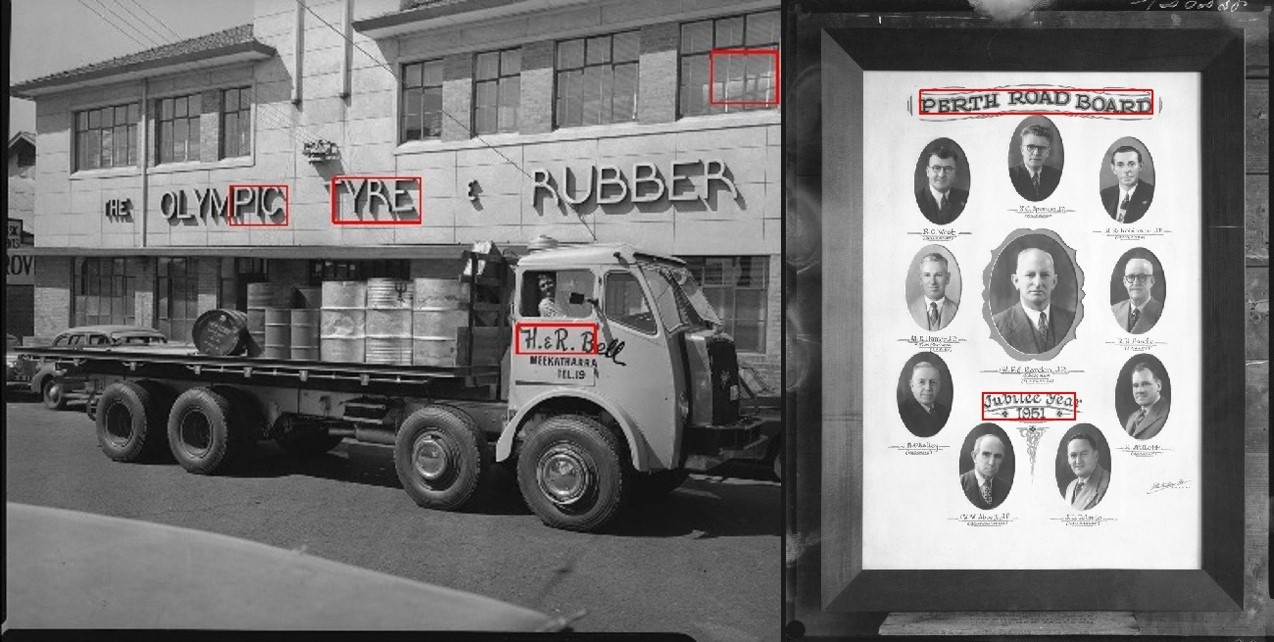
\includegraphics[width=\columnwidth]{figures/text_recognition.jpg}
  \caption{Two photographs processed with Thickshake's text recognition algorithm. Red boxes are the bounding boxes of each detected text region.}
  \label{figure:text_recognition:images}
\end{figure}

\section{Machine Learning}
\label{section:machine_learning}

%\subsection{Introduction}
\label{subsection:machine_learning:introduction}
Metadata parsing and image processing are performed on a per-record basis, and we can gain even more insights by identifying trends across the catalogue using machine learning. We developed a machine learning framework that is designed for a distributed, high-performance computing environment, specifically, Pawsey Supercomputing Centre’s Athena GPU cluster. Machine learning predictions are stored in a parallel-access HDF5 store which our system syncs with the main relational database. The framework is built around a dependency manager that allows metadata parsers, image processors and machine learning algorithms to build on each other to generate more complicated metadata. The first machine learning function we started developing was a subject recognition classifier that synthesises face detection results with existing metadata from the catalogue. We plan to continue developing this and other classifiers in the future.

\subsection{Parallel Datastore}
\label{subsection:machine_learning:parallel_datastore}
Handling parallel IO operations is one of the more challenging aspects of working in a high-performance computing environment. To manage the intermediate data from our image processing and machine learning algorithms, we used HDF5, a hierarchical data format designed to store and organize large amounts of data \cite{hdf5}. Specifically, we used PyTables, a Python wrapper for HDF5 that provides a Pandas-like interface for the underlying data arrays \cite{pytables}. This library facilitates intuitive and structured queries  while still providing lazy and parallel read and write operations. Each image processing or machine learning function stores their data in a separate dataframe under the hierarchical structure, and multiple threads can append or extract records from the dataframes in parallel. These dataframes are transformed and copied into the relational database as the operations are completed.

\subsection{Dependency Manager}
\label{subsection:machine_learning:dependency_manager}
Metadata parsing, image processing, and machine learning all have the capacity to create new attributes and records in the relational database. We can generate richer data by layering multiple augmentation functions. To do this, we created a dependency manager. The dependency manager checks and invokes all missing dependency functions and sync operations to ensure that the given function runs cleanly with access to all relevant intermediate results. The dependency manager performs checks at two levels: first, it checks whether a given functions' dependencies' results have been stored in the parallel datastore; second, it checks whether those results have also been synced to the relational database. The details of which data from the datastore has been synced to the database is stored in a table in the database that acts as a ledger: it stores the type of function performed, the timestamp when the function was first performed and the timestamp of when it was most recently performed. This allows the program to check whether the intermediate results are available and how timely they are. Figure \ref{figure:dependency_manager} provides an illustrative workflow that could be performed by the dependency manager.

\begin{figure}[ht]
  \centering
  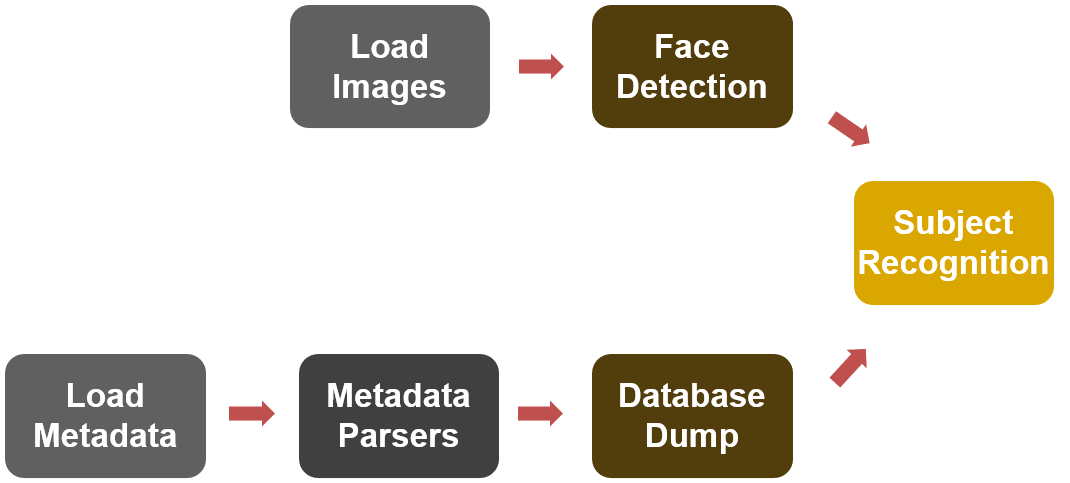
\includegraphics[width=\columnwidth]{figures/dependency_manager.png}
  \caption{Subject recognition workflow used by the dependency manager.}
  \label{figure:dependency_manager}
\end{figure}

\subsection{Subject Recognition}
\label{subsection:machine_learning:subject_recognition}
Subject recognition is a highly valuable description task for archival images but also one of the most challenging tasks for humans. Building on our face detection algorithm, we started to develop an automated subject recognition function. Our subject recognition system has multiple stages: 1. pre-process the image, 2. identify facial bounding boxes 3. identify facial landmarks, 4. generate facial embeddings, 5. combine metadata and facial embeddings, 6. train the neural network, 7. apply the trained neural network to make predictions. Stages 1 and 2 together are our face detection algorithm (see Section \ref{subsection:image_processing:face_detection}). Stage 3 used a dlib function to generate facial landmarks (e.g. tip of nose, points of mouth) from the identified faces \cite{dlib_face}. Stage 4 uses a dlib neural network that can convert the facial landmarks into embeddings that uniquely identify each person \cite{he2016}.These embeddings are stored into the parallel datastore. In stage 5, the dependency manager ensures that the metadata parsers have been run and the relational database has been dumped to the paralle data store. It then joins the metadata with the facial embeddings by image id. We then feed this combined flat file into Tensorflow in stage 6 and 7.

Unfortunately, we were unable to get the machine learning system working to our satisfaction by the end of the project due to time constraints. A key challenge we faced was the format of the \Gls{slwa} records: subject labels are documented on a per-record basis, not a per-image basis (records often contain multiple closely-related images). Therefore, the vast majority of provided subject labels were ambiguous/fuzzy. Combine this with the complications of 2,036 labels (people) in our test dataset, and a highly skewed label distribution (most people only appeared one or two times), and supervised machine learning is very difficult. We briefly investigated semi-supervised learning, treating subjects with conflicting labels as unlabelled, and extrapolating from the structure of the unambiguous labels. This was also unsuccessful, due to the small percentage of unambiguous labels. We still believe that machine learning can be applied to this problem, but it will likely require a much larger test dataset to achieve satisfactory results.

\section{Conclusions}
\label{section:conclusions}
There are many potential opportunities for future work extending this project. Completing the MARC exporter facility will allow this project's augmented metadata to feed back into the library catalogue. Text recognition and subject recognition remain unsolved by this project but much of the groundwork has already been achieved. Image captioning \cite{karpathy2015} and landmark recognition \cite{ardeshir2015} are also interesting extensions that have had some success in other domains. Finally, building clustering, similarity and improved search algorithms on top of Thickshake could make a huge difference to the usability of library catalogues, answering questions like "Which images in the catalogue are most important?" or "What other images depict this person?".

This project makes three primary contributions: 1. An extensible and flexible platform for manipulating and augmenting library catalogue metadata. 2. A suite of processing functions including geolocation, face detection, text recognition, and others. 3. A system that leverages cutting-edge image processing and machine learning libraries on Pawsey Supercomputing Centre’s Athena GPU cluster. 

\section{Acknowledgements}
\label{section:acknowledgements}
We wish to acknowledge and thank the following groups and individuals for their support of the project: The State Library of Western Australia, particularly Adrian Bowen, Catherine Kelso, and Barbara Patison, for the provision of records from the photographic archive of the Battye Library of West Australian History and other supervisory guidance. The Pawsey Supercomputing Centre, and particularly Maciej Cytowski, for the provision of supercomputing services and technical support. This work was supported by resources provided by The Pawsey Supercomputing Centre with funding from the Australian Government and the Government of Western Australia. This work was also supported by the Curtin HIVE and the State Library of Western Australia.

\printbibliography

\pagebreak\clearpage\appendix

\section{MARC Input Map}
\label{appendix:marc_input_map}
\inputminted{yaml}{appendices/input.yaml}

\section{MARC Output Map}
\label{appendix:marc_output_map}
\inputminted{yaml}{appendices/output.yaml}

\pagebreak

\section{Database Schema}
\label{appendix:database_schema}
\inputminted{yaml}{appendices/schema.yaml}

\pagebreak
\onecolumn

\section{Command Line Interface}
\label{appendix:command_line_interface}
\subsection{Commands}

\begin{minted}{bash}
  thickshake load # Imports a catalogue file into the database (MARC, XML, JSON).

  thickshake augment caption_images # Automatically captions images. [TODO]
  thickshake augment detect_faces # Detects faces in images.
  thickshake augment identify_faces # Identifies faces in images. [TODO]
  thickshake augment read_text # Reads text embedded in images. [TODO]
  thickshake augment parse_dates # Parses dates from text fields.
  thickshake augment parse_links # Parses links from text fields.
  thickshake augment parse_locations # Parses locations from text fields.
  thickshake augment parse_sizes # Parses image sizes from urls.
  thickshake augment run_all # Runs all augment functions.
  thickshake augment run_parsers # Runs all metadata parsing functions.
  thickshake augment run_processors # Runs all image processing functions.

  thickshake export query # Exports a report from the database (CSV, JSON).
  thickshake export dump # Exports a flat file from the database (CSV, JSON).
  thickshake export marc # Exports a catalogue file from the database(MARC, XML, JSON). [WIP]

  thickshake inspect # Inspects the state of the database (lists tables and number of records).
  thickshake convert # Converts a catalogue file between formats (MARC, XML, JSON).
\end{minted}

\subsection{Shared Options}

\begin{itemize}
  \item "-f", "--force", help="overwrite existing files"
  \item "-d", "--dry-run", help="run without writing files"
  \item "-g", "--graphics", help="display images in GUI"
  \item "-s", "--sample", help="perform on random sample (default: 0 / None)"
  \item "-v", "--verbosity", help="either CRITICAL, ERROR, WARNING, INFO or DEBUG"
\end{itemize}

\pagebreak

\section{Docker Automated Build}
\label{appendix:docker_automated_build}
\subsection{Installation}

Install Docker on your machine as described in the \href{http://docs.docker.com/engine/installation/}{Docker documentation}.

\begin{minted}{bash}
  git clone https://github.com/markshelton/thickshake
  cd thickshake
  make start ENV=dev # development
  make start ENV=prod # production
\end{minted}

\subsection{Containers}

\begin{description}
    \item[App Container (Image: \href{https://hub.docker.com/r/markshelton/thickshake/}{markshelton/thickshake})]
\end{description}

\begin{itemize}
  \item Python 3.5
  \item Tensorflow 1.4.0
  \item OpenCV 3.3.1
  \item dlib 19.7
\end{itemize}

\begin{description}
    \item[Database Container (Image: \href{https://hub.docker.com/_/postgres/}{postgres})]
\end{description}

\begin{itemize}
  \item PostgreSQL 10.1
\end{itemize}

\subsection{Make Commands}

\begin{minted}{bash}
  make start # loads and builds images, creates data volume, creates virtual network, opens shell
  make stop # saves python environment, stops containers, removes virtual network
  make restart # stops and restarts containers and virtual network
  make jupyter # opens jupyter service in default internet browser
  make shell # opens interactive session with app container
  make push # tags app image and pushes image to DockerHub
\end{minted}

\end{document}
